\clearpage\begingroup\SourceLeaf{59}\HistoricalHead{54}{L}{PHYSIK. BRIEFWECHSEL.}
\begin{center}
[7.]\\[.7em]
\textsc{Schumacher} an \textsc{Gauss}. Altona, 1830, Januar 5.
\par\smallskip\rule{.78\textwidth}{.35pt}\\
{\small [Briefwechsel zwischen \textsc{Gauss} und \textsc{Schumacher} II, Altona 1860, S. 221.]}\\
\rule{.78\textwidth}{.35pt}
\end{center}
\noindent\hspace*{\parindent}\{Anbei erhalten Sie, mein theuerster Freund!
\begin{list}{}{\setlength{\leftmargin}{1.8em}\setlength{\labelwidth}{1.3em}\setlength{\labelsep}{.5em}\setlength{\listparindent}{1.2em}\setlength{\itemsep}{.3em}\setlength{\topsep}{0pt}}
\item[1)] \textsc{Pritshards} Saphirlinse. Sie ist durch einen übergeschraubten Messingdeckel
verwahrt.
\item[2)] \textsc{Dollonds} Stand dazu, dessen einfacher Mechanismus keiner Erklärung
bedarf, nebst einem Planglas, um darauf ein Tröpfchen irgend einer feinst
möglich zerriebenen in Wasser aufgelösten Materie zu thun.
\item[3)] Ein Test-Object, was zu den schwierigsten Proben der Microscope gehört.
Es ist eine Schuppe von den Flügeln des gelben Kohlschmetterlings zwischen
Glas und Marienglas. Die Seite mit Marienglas muss natürlich
gegen das Microscop gewandt seyn, weil man sonst nicht wegen der Dicke
des Glases nahe genug kommen kann.

Sie erscheint \raisebox{-.6em}{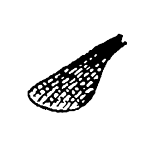
\begin{tikzpicture}[x=.1bp,y=-.1bp,baseline=-.5ex]
\fill[black] (376,50) -- (374,48) -- (372,48) -- (370,46) -- (366,46) -- (365,44) -- (359,44) -- (357,46) -- (357,48) -- (354,51) -- (352,51) -- (348,55) -- (343,55) -- (341,57) -- (339,57) -- (336,60) -- (332,60) -- (330,62) -- (328,62) -- (327,64) -- (325,64) -- (323,66) -- (321,66) -- (318,69) -- (316,69) -- (312,73) -- (310,73) -- (307,76) -- (303,76) -- (302,78) -- (300,78) -- (298,80) -- (294,80) -- (292,82) -- (289,82) -- (286,85) -- (285,85) -- (284,87) -- (280,87) -- (278,89) -- (276,89) -- (263,102) -- (258,102) -- (252,108) -- (252,110) -- (250,112) -- (246,112) -- (238,120) -- (231,120) -- (228,123) -- (226,123) -- (217,132) -- (213,132) -- (213,133) -- (211,134) -- (210,136) -- (209,136) -- (206,139) -- (204,139) -- (203,141) -- (201,141) -- (199,143) -- (195,143) -- (186,152) -- (182,152) -- (182,153) -- (178,157) -- (177,157) -- (176,159) -- (170,159) -- (168,161) -- (166,161) -- (165,163) -- (161,163) -- (154,170) -- (152,170) -- (147,175) -- (145,175) -- (141,179) -- (139,179) -- (139,180) -- (137,181) -- (132,186) -- (127,186) -- (121,192) -- (117,192) -- (116,193) -- (114,193) -- (114,194) -- (112,195) -- (112,196) -- (110,197) -- (110,198) -- (108,199) -- (107,201) -- (102,202) -- (98,206) -- (96,206) -- (94,208) -- (90,208) -- (89,210) -- (87,210) -- (84,213) -- (80,213) -- (78,215) -- (76,215) -- (76,216) -- (74,217) -- (71,220) -- (68,220) -- (57,231) -- (53,231) -- (42,242) -- (42,244) -- (40,246) -- (38,246) -- (33,251) -- (33,268) -- (35,270) -- (36,275) -- (38,276) -- (38,278) -- (40,280) -- (40,282) -- (53,295) -- (55,295) -- (59,299) -- (61,299) -- (63,301) -- (63,302) -- (64,302) -- (65,304) -- (67,305) -- (67,306) -- (75,306) -- (78,309) -- (80,309) -- (81,311) -- (84,311) -- (85,313) -- (87,313) -- (89,315) -- (95,315) -- (96,317) -- (98,317) -- (100,315) -- (102,315) -- (104,317) -- (106,317) -- (110,320) -- (114,320) -- (116,322) -- (118,322) -- (120,324) -- (134,324) -- (136,326) -- (138,326) -- (139,327) -- (147,327) -- (148,326) -- (154,326) -- (155,327) -- (160,327) -- (161,326) -- (175,326) -- (177,324) -- (181,324) -- (182,322) -- (201,322) -- (202,320) -- (205,320) -- (205,319) -- (207,317) -- (215,317) -- (219,313) -- (221,313) -- (221,312) -- (223,311) -- (223,310) -- (225,308) -- (227,308) -- (229,306) -- (233,306) -- (235,304) -- (237,304) -- (237,303) -- (239,302) -- (244,297) -- (244,296) -- (246,295) -- (246,294) -- (248,293) -- (253,288) -- (253,287) -- (255,286) -- (255,285) -- (257,284) -- (262,279) -- (263,277) -- (264,277) -- (265,275) -- (266,275) -- (266,271) -- (268,269) -- (268,267) -- (273,262) -- (273,260) -- (275,259) -- (276,257) -- (277,257) -- (277,249) -- (278,248) -- (278,245) -- (280,243) -- (280,241) -- (282,239) -- (282,235) -- (284,233) -- (284,231) -- (286,230) -- (286,226) -- (287,225) -- (287,223) -- (289,221) -- (289,219) -- (291,217) -- (291,213) -- (293,212) -- (293,208) -- (295,206) -- (295,202) -- (298,198) -- (298,192) -- (300,190) -- (300,186) -- (302,185) -- (302,181) -- (304,179) -- (304,175) -- (307,171) -- (307,169) -- (309,167) -- (309,165) -- (313,161) -- (313,157) -- (316,153) -- (316,151) -- (318,149) -- (318,147) -- (320,145) -- (320,143) -- (326,137) -- (328,137) -- (331,134) -- (332,129) -- (334,128) -- (335,126) -- (336,126) -- (336,123) -- (338,122) -- (343,117) -- (343,116) -- (345,115) -- (346,113) -- (349,113) -- (349,112) -- (351,110) -- (352,110) -- (352,109) -- (354,108) -- (354,107) -- (356,106) -- (357,104) -- (359,104) -- (370,93) -- (375,92) -- (384,83) -- (388,83) -- (388,82) -- (390,81) -- (390,75) -- (386,71) -- (380,71) -- (380,72) -- (376,76) -- (375,76) -- (370,71) -- (370,68) -- (372,66) -- (372,60) -- (374,59) -- (374,55) -- (376,53) -- cycle;
\fill[white] (218,303) -- (218,306) -- (215,309) -- (211,309) -- (208,312) -- (204,312) -- (203,314) -- (193,314) -- (192,316) -- (186,316) -- (185,314) -- (183,313) -- (183,311) -- (192,302) -- (192,300) -- (204,288) -- (206,288) -- (213,295) -- (213,298) -- (209,302) -- (209,304) -- (213,304) -- (215,302) -- (217,302) -- cycle;
\fill[white] (236,282) -- (238,284) -- (238,286) -- (236,287) -- (236,288) -- (233,292) -- (231,292) -- (228,289) -- (228,287) -- (230,286) -- (231,284) -- (233,284) -- (235,282) -- cycle;
\fill[white] (213,279) -- (215,279) -- (218,282) -- (218,288) -- (217,289) -- (215,289) -- (210,284) -- (210,282) -- cycle;
\fill[white] (187,282) -- (190,279) -- (190,278) -- (192,277) -- (193,275) -- (199,275) -- (200,277) -- (202,278) -- (202,282) -- (199,285) -- (197,285) -- (195,287) -- (191,287) -- (190,285) -- cycle;
\fill[white] (117,272) -- (118,272) -- (126,280) -- (126,282) -- (123,285) -- (122,287) -- (118,287) -- (115,284) -- (115,282) -- (113,280) -- (113,276) -- (115,275) -- (115,274) -- cycle;
\fill[white] (241,261) -- (242,262) -- (242,265) -- (240,267) -- (240,268) -- (238,269) -- (238,270) -- (236,271) -- (231,276) -- (231,277) -- (229,278) -- (228,280) -- (224,280) -- (221,277) -- (221,273) -- (223,271) -- (223,269) -- (226,266) -- (228,266) -- (230,264) -- (232,264) -- (233,263) -- (236,263) -- (238,261) -- cycle;
\fill[white] (139,257) -- (144,262) -- (144,264) -- (141,267) -- (141,268) -- (139,269) -- (138,271) -- (137,271) -- (134,274) -- (132,274) -- (127,269) -- (127,262) -- (129,261) -- (129,260) -- (131,259) -- (132,257) -- cycle;
\fill[white] (224,248) -- (227,251) -- (227,257) -- (210,274) -- (206,274) -- (203,271) -- (202,271) -- (201,270) -- (201,267) -- (207,263) -- (209,263) -- (215,257) -- (215,255) -- (217,254) -- (217,253) -- (219,252) -- (219,251) -- (221,250) -- (222,248) -- cycle;
\fill[white] (196,246) -- (197,246) -- (200,249) -- (200,250) -- (201,250) -- (202,252) -- (204,253) -- (204,257) -- (202,258) -- (202,259) -- (200,260) -- (199,262) -- (197,262) -- (192,257) -- (192,249) -- cycle;
\fill[white] (146,245) -- (147,245) -- (152,250) -- (152,253) -- (150,255) -- (147,255) -- (143,251) -- (143,248) -- cycle;
\fill[white] (170,246) -- (172,245) -- (173,243) -- (176,243) -- (182,248) -- (182,250) -- (179,253) -- (175,253) -- (174,251) -- (172,250) -- (172,247) -- cycle;
\fill[white] (270,242) -- (270,245) -- (268,247) -- (264,247) -- (262,249) -- (260,249) -- (253,256) -- (242,256) -- (239,253) -- (247,245) -- (249,245) -- (253,241) -- (255,241) -- (256,239) -- (267,239) -- cycle;
\fill[white] (236,238) -- (237,238) -- (240,241) -- (238,242) -- (237,244) -- (235,244) -- (233,242) -- (233,241) -- cycle;
\fill[white] (203,239) -- (206,236) -- (212,236) -- (216,240) -- (216,245) -- (214,247) -- (207,247) -- (205,245) -- (205,244) -- (203,243) -- cycle;
\fill[white] (101,236) -- (106,236) -- (110,240) -- (110,243) -- (106,247) -- (101,247) -- (98,244) -- (98,239) -- cycle;
\fill[white] (188,296) -- (186,298) -- (186,300) -- (184,302) -- (184,304) -- (182,305) -- (182,306) -- (176,312) -- (175,312) -- (175,315) -- (171,318) -- (161,318) -- (160,316) -- (148,316) -- (146,318) -- (140,318) -- (138,316) -- (125,316) -- (121,312) -- (114,312) -- (111,309) -- (107,309) -- (106,307) -- (102,307) -- (100,305) -- (94,305) -- (93,303) -- (89,303) -- (87,301) -- (80,301) -- (77,298) -- (73,298) -- (67,292) -- (63,292) -- (61,290) -- (61,289) -- (60,289) -- (59,287) -- (58,287) -- (57,285) -- (56,285) -- (55,283) -- (54,283) -- (52,281) -- (52,280) -- (51,280) -- (50,278) -- (49,278) -- (48,276) -- (47,276) -- (46,274) -- (45,274) -- (43,272) -- (43,266) -- (39,262) -- (39,258) -- (41,257) -- (46,252) -- (51,252) -- (53,250) -- (53,245) -- (55,243) -- (55,242) -- (57,241) -- (58,239) -- (60,239) -- (62,241) -- (64,241) -- (67,244) -- (67,246) -- (62,251) -- (62,256) -- (60,258) -- (60,259) -- (58,260) -- (57,262) -- (54,262) -- (53,264) -- (53,270) -- (59,270) -- (61,272) -- (62,272) -- (62,267) -- (61,265) -- (65,261) -- (67,261) -- (69,259) -- (71,259) -- (75,263) -- (80,263) -- (82,261) -- (82,258) -- (77,253) -- (77,251) -- (82,246) -- (84,246) -- (85,245) -- (89,245) -- (92,248) -- (93,248) -- (94,250) -- (96,251) -- (96,255) -- (91,260) -- (89,260) -- (72,277) -- (72,279) -- (69,282) -- (69,284) -- (67,285) -- (67,288) -- (68,288) -- (69,290) -- (71,288) -- (76,288) -- (79,285) -- (79,283) -- (81,281) -- (82,281) -- (82,278) -- (84,277) -- (84,276) -- (88,273) -- (88,271) -- (93,266) -- (96,266) -- (100,270) -- (102,270) -- (102,269) -- (104,268) -- (104,266) -- (102,264) -- (102,260) -- (104,259) -- (104,258) -- (106,257) -- (107,255) -- (109,255) -- (114,250) -- (118,250) -- (122,246) -- (122,242) -- (125,239) -- (127,239) -- (129,237) -- (131,237) -- (136,232) -- (140,232) -- (141,234) -- (143,234) -- (144,235) -- (144,239) -- (141,242) -- (134,242) -- (134,244) -- (132,246) -- (132,248) -- (130,249) -- (130,250) -- (128,251) -- (128,252) -- (124,256) -- (123,256) -- (123,257) -- (121,258) -- (121,259) -- (119,260) -- (119,261) -- (113,267) -- (112,267) -- (112,268) -- (110,269) -- (109,271) -- (107,271) -- (105,273) -- (105,275) -- (103,276) -- (103,277) -- (101,278) -- (101,279) -- (95,285) -- (94,285) -- (94,286) -- (92,287) -- (91,289) -- (89,289) -- (87,291) -- (87,297) -- (89,299) -- (91,297) -- (93,297) -- (93,296) -- (95,295) -- (95,294) -- (97,293) -- (98,291) -- (109,291) -- (111,290) -- (114,293) -- (114,300) -- (112,302) -- (112,304) -- (113,304) -- (114,306) -- (116,306) -- (122,300) -- (122,298) -- (124,296) -- (124,294) -- (127,291) -- (130,291) -- (132,293) -- (134,293) -- (136,291) -- (136,289) -- (138,288) -- (139,286) -- (143,286) -- (145,284) -- (145,282) -- (140,277) -- (140,276) -- (142,275) -- (142,274) -- (144,272) -- (145,272) -- (145,269) -- (147,268) -- (147,267) -- (149,266) -- (154,261) -- (154,260) -- (156,259) -- (156,258) -- (158,257) -- (163,252) -- (167,252) -- (171,256) -- (171,263) -- (167,267) -- (166,267) -- (166,268) -- (164,269) -- (164,270) -- (161,273) -- (160,273) -- (158,271) -- (156,271) -- (154,269) -- (152,269) -- (150,271) -- (150,275) -- (152,277) -- (152,283) -- (150,285) -- (150,287) -- (144,293) -- (144,295) -- (136,303) -- (136,304) -- (138,306) -- (143,306) -- (145,304) -- (145,302) -- (147,300) -- (147,298) -- (154,291) -- (157,291) -- (159,293) -- (163,293) -- (163,289) -- (161,287) -- (161,281) -- (163,279) -- (163,278) -- (165,277) -- (165,276) -- (167,275) -- (172,270) -- (173,268) -- (174,268) -- (175,266) -- (176,266) -- (180,263) -- (183,263) -- (189,269) -- (189,270) -- (186,273) -- (184,273) -- (182,275) -- (182,280) -- (180,282) -- (180,284) -- (177,287) -- (175,287) -- (174,285) -- (172,284) -- (172,283) -- (170,283) -- (168,285) -- (168,288) -- (171,291) -- (171,295) -- (170,296) -- (170,298) -- (159,309) -- (159,311) -- (161,313) -- (176,298) -- (176,296) -- (178,294) -- (178,292) -- (180,290) -- (185,290) -- (188,293) -- cycle;
\fill[white] (82,227) -- (85,230) -- (85,232) -- (87,233) -- (87,235) -- (82,240) -- (80,240) -- (76,244) -- (75,244) -- (71,240) -- (71,238) -- (70,237) -- (70,231) -- (71,230) -- (73,230) -- (75,228) -- (77,228) -- (78,227) -- cycle;
\fill[white] (179,225) -- (179,228) -- (176,231) -- (174,231) -- (167,238) -- (163,238) -- (159,242) -- (157,242) -- (156,241) -- (156,237) -- (158,235) -- (158,233) -- (164,227) -- (168,227) -- (174,221) -- (175,221) -- cycle;
\fill[white] (88,220) -- (90,218) -- (95,218) -- (101,224) -- (101,226) -- (98,229) -- (94,229) -- (88,223) -- cycle;
\fill[white] (240,219) -- (240,224) -- (236,228) -- (234,228) -- (233,229) -- (224,229) -- (221,226) -- (221,224) -- (226,219) -- (228,219) -- (231,216) -- (237,216) -- cycle;
\fill[white] (213,219) -- (213,221) -- (211,222) -- (211,223) -- (209,224) -- (209,225) -- (203,231) -- (201,231) -- (188,244) -- (184,244) -- (183,242) -- (182,242) -- (179,238) -- (179,236) -- (182,232) -- (185,232) -- (185,231) -- (187,230) -- (187,229) -- (189,227) -- (191,227) -- (195,223) -- (197,223) -- (199,221) -- (203,221) -- (208,216) -- (210,216) -- cycle;
\fill[white] (264,214) -- (265,216) -- (266,216) -- (269,219) -- (266,222) -- (265,222) -- (265,223) -- (263,224) -- (262,226) -- (260,226) -- (251,235) -- (248,235) -- (244,231) -- (244,228) -- (258,214) -- cycle;
\fill[white] (143,212) -- (144,213) -- (144,219) -- (141,222) -- (139,222) -- (139,223) -- (137,224) -- (136,226) -- (132,226) -- (125,233) -- (123,233) -- (118,228) -- (118,226) -- (120,225) -- (120,224) -- (122,223) -- (123,221) -- (127,221) -- (129,219) -- (133,219) -- (136,216) -- (136,215) -- (138,214) -- (139,212) -- cycle;
\fill[white] (122,205) -- (125,209) -- (125,210) -- (123,211) -- (123,212) -- (121,213) -- (120,215) -- (118,215) -- (116,217) -- (114,217) -- (111,220) -- (108,220) -- (106,218) -- (106,213) -- (110,209) -- (112,209) -- (114,207) -- (116,207) -- (118,205) -- cycle;
\fill[white] (205,206) -- (204,208) -- (204,210) -- (201,213) -- (199,213) -- (195,217) -- (193,217) -- (190,220) -- (184,220) -- (183,219) -- (183,217) -- (184,216) -- (186,216) -- (193,209) -- (195,209) -- (201,203) -- (202,203) -- cycle;
\fill[white] (228,203) -- (229,204) -- (229,207) -- (227,208) -- (222,213) -- (220,213) -- (217,210) -- (217,206) -- (219,205) -- (220,203) -- (224,203) -- (225,202) -- cycle;
\fill[white] (182,204) -- (182,208) -- (177,213) -- (176,215) -- (173,215) -- (172,217) -- (170,217) -- (167,220) -- (165,220) -- (163,222) -- (159,222) -- (156,219) -- (156,217) -- (163,210) -- (168,209) -- (174,203) -- (176,203) -- (178,201) -- (179,201) -- cycle;
\fill[white] (255,200) -- (258,203) -- (258,206) -- (256,208) -- (254,208) -- (251,211) -- (247,211) -- (246,210) -- (246,204) -- (248,203) -- (251,200) -- cycle;
\fill[white] (164,201) -- (159,206) -- (155,206) -- (154,205) -- (154,203) -- (157,200) -- (159,200) -- (161,198) -- cycle;
\fill[white] (283,192) -- (287,196) -- (287,202) -- (284,206) -- (276,206) -- (274,208) -- (273,208) -- (270,205) -- (270,204) -- (282,192) -- cycle;
\fill[white] (149,187) -- (151,191) -- (149,193) -- (145,193) -- (141,197) -- (141,201) -- (138,204) -- (134,204) -- (131,201) -- (131,197) -- (134,194) -- (136,194) -- (139,191) -- (143,191) -- (146,187) -- cycle;
\fill[white] (254,184) -- (254,187) -- (248,193) -- (246,193) -- (242,197) -- (240,197) -- (238,199) -- (237,199) -- (235,197) -- (235,192) -- (242,185) -- (244,185) -- (246,183) -- (253,183) -- cycle;
\fill[white] (277,182) -- (279,184) -- (279,187) -- (267,199) -- (266,199) -- (260,193) -- (260,192) -- (262,191) -- (262,190) -- (264,189) -- (264,188) -- (266,187) -- (267,185) -- (269,185) -- (272,182) -- cycle;
\fill[white] (232,182) -- (233,184) -- (231,186) -- (231,187) -- (229,188) -- (229,189) -- (227,190) -- (222,195) -- (222,196) -- (220,197) -- (219,199) -- (218,199) -- (215,202) -- (213,202) -- (210,199) -- (210,195) -- (212,194) -- (217,189) -- (218,187) -- (221,187) -- (222,185) -- (224,185) -- (227,182) -- cycle;
\fill[white] (267,169) -- (270,172) -- (270,174) -- (267,177) -- (267,178) -- (265,179) -- (264,181) -- (260,181) -- (257,178) -- (257,174) -- (260,171) -- (262,171) -- (263,169) -- cycle;
\fill[white] (177,169) -- (180,172) -- (180,174) -- (177,177) -- (177,178) -- (175,179) -- (175,180) -- (171,183) -- (169,183) -- (167,181) -- (166,181) -- (165,180) -- (165,176) -- (168,173) -- (170,173) -- (173,169) -- cycle;
\fill[white] (289,167) -- (294,167) -- (297,170) -- (297,174) -- (294,177) -- (293,179) -- (287,179) -- (284,176) -- (284,172) -- cycle;
\fill[white] (231,170) -- (231,172) -- (228,175) -- (226,175) -- (218,183) -- (216,183) -- (213,186) -- (212,188) -- (209,188) -- (209,189) -- (206,192) -- (203,192) -- (201,190) -- (201,186) -- (203,185) -- (208,180) -- (208,179) -- (210,178) -- (211,176) -- (214,176) -- (214,175) -- (218,171) -- (219,171) -- (220,169) -- (222,169) -- (224,167) -- (228,167) -- (229,169) -- cycle;
\fill[white] (211,168) -- (211,171) -- (210,172) -- (209,172) -- (206,175) -- (203,175) -- (195,183) -- (190,184) -- (186,188) -- (183,188) -- (181,186) -- (181,183) -- (184,180) -- (186,180) -- (193,173) -- (195,173) -- (197,171) -- (199,171) -- (199,170) -- (201,169) -- (202,167) -- (205,167) -- (206,165) -- (208,165) -- (209,167) -- cycle;
\fill[white] (257,162) -- (258,163) -- (258,165) -- (253,170) -- (251,170) -- (247,174) -- (246,174) -- (244,172) -- (244,170) -- (246,169) -- (247,167) -- (250,167) -- (250,166) -- (252,164) -- (253,164) -- (254,162) -- cycle;
\fill[white] (246,155) -- (249,158) -- (247,159) -- (247,160) -- (245,161) -- (245,162) -- (241,166) -- (238,166) -- (235,163) -- (235,161) -- (237,160) -- (237,159) -- (241,156) -- (244,156) -- cycle;
\fill[white] (219,158) -- (222,155) -- (228,155) -- (229,156) -- (226,159) -- (224,159) -- (222,161) -- cycle;
\fill[white] (287,151) -- (290,154) -- (290,156) -- (283,163) -- (278,163) -- (277,162) -- (277,157) -- (279,155) -- (281,155) -- (285,151) -- cycle;
\fill[white] (246,140) -- (247,141) -- (247,144) -- (245,145) -- (240,150) -- (238,150) -- (235,147) -- (242,140) -- cycle;
\fill[white] (312,133) -- (315,136) -- (315,137) -- (312,140) -- (312,142) -- (310,143) -- (310,144) -- (308,145) -- (305,148) -- (300,143) -- (300,141) -- (302,140) -- (307,135) -- (309,135) -- (310,133) -- cycle;
\fill[white] (262,129) -- (263,131) -- (265,132) -- (265,133) -- (263,134) -- (263,135) -- (260,138) -- (259,138) -- (255,134) -- (257,133) -- (257,132) -- (259,131) -- (260,129) -- cycle;
\fill[white] (280,117) -- (283,120) -- (276,127) -- (275,127) -- (273,125) -- (273,122) -- (278,117) -- cycle;
\end{tikzpicture}
} aus Langstreifen zusammengesetzt, die Punkte
haben.
\item[4)] In einer blechernen Büchse eine Auflösung von Gummigutt in Wasser
zwischen Glas und Marienglas, und durch Oelfirniss luftdicht verschlossen,
den \textsc{Nehus} vor etwa 3 Monaten in London gekauft hat (bei \textsc{Cary}). Es
soll dadurch bewiesen werden, dass durch das Verdunsten des Wassers die
Bewegung der Atome \textls[120]{nicht} hervorgebracht wird, und es hält auch den
Einfluss localer Bewegungen durch Temperaturveränderungen mehr ab, als
wenn der Tropfen offen wäre. Obgleich man in London glaubte, diese
Vorrichtung könne die Bewegung der Atome auf 14 Tage sichern, so ist
sie noch jetzt an mehreren Stellen ebenso lebhaft darin, wie im Anfange.
An anderen Stellen hingegen, die wahrscheinlich aufgetrocknet sind, ist
alles todt. Sie werden leicht die lebendigen (oder besser beweglichen)
Atome ausfinden.\quad \mbox{.\ .\ .\ .\ .\ .\ .\ .\ .\ .\ .\ .\ .\ .\ .\ .\ .\ .\ .\ .\ .\}}
\end{list}
\begin{center}\rule{.18\textwidth}{.35pt}\end{center}
\HistoricalHead{54}{L}{PHYSIK. BRIEFWECHSEL.}\clearpage\endgroup
